\documentclass[conference]{IEEEtran}
\IEEEoverridecommandlockouts
% The preceding line is only needed to identify funding in the first footnote. If that is unneeded, please comment it out.
%Template version as of 6/27/2024
\usepackage{tikz}
\usetikzlibrary{positioning, shapes, arrows.meta}
\usepackage{cite}
\usepackage{amsmath,amssymb,amsfonts}
\usepackage{algorithmic}
\usepackage{graphicx}
\usepackage{textcomp}
\usepackage{xcolor}
\usepackage[hidelinks]{hyperref}
\def\BibTeX{{\rm B\kern-.05em{\sc i\kern-.025em b}\kern-.08em
    T\kern-.1667em\lower.7ex\hbox{E}\kern-.125emX}}
\begin{document}

\title{S(oC)DR: A Low Cost, SoC-Based Software Defined Radio Platform\\
}

\author{\IEEEauthorblockN{Ajay Thakkar}
\IEEEauthorblockA{\textit{Electrical and Computer Engineering} \\
\textit{Stevens Institute of Technology}\\
Hoboken, New Jersey \\
athakka5@stevens.edu}
\and
\IEEEauthorblockN{Bernard Yett}
\IEEEauthorblockA{\textit{Electrical and Computer Engineering} \\
\textit{Stevens Institute of Technology}\\
Hoboken, New Jersey \\
byett@stevens.edu}
}

\maketitle

\section{Introduction}
Modern RF systems require portability and computational power to solve complex problems in dynamic environments.
Applications like remote sensing and tactical communications require self sufficient RF systems that can operate on the edge while employing
modern algorithms such as spectrum sensing and signal classification. Creating such devices usually requires
custom hardware and software that are tailored to the application, which is both a costly and non-reusable solution \cite{10880410}. Technology such as
Software Defined Radios (SDR) and System-on-Chips (SoC) can be leveraged in these applications to form fast, reprogrammable, portable, and cost effective systems \cite{9721283}.

SDRs are flexible RF systems that allow for digital reconfigurability to change its operational parameters while running.
Their novelty lies in the interface between a General-Purpose Processor (GPP) and an RF front end, allowing the user to digitally control the front end's
operating frequency, gain, sampling rate, etc. This GPP also allows for a personal computer to communicate with the system to send commands and retrieve return
data for further processing \cite{9721283}. Software such as GNU Radio and MATLAB include packages to communicate with popular SDRs as well as signal processing and visualization
blocks that can be tailored to a wide variety of RF tasks. This SDR ecosystem has been used extensively in modern research for prototyping RF systems,
like Hu et al. utilizing the Pluto SDR platform as well as MATLAB's deep learning toolbox to implement a Convolutional Neural Network (CNN) 
for signal classification of the Pluto SDR's return signal \cite{9687958}. However, since many of these studies use a personal computer for their data processing which have a large form factor 
and utilize a lot of power, these systems are not viable for field testing or deployment. 

To that end, many of these same signal processing applications such as CNNs have been
implemented on programmable logic platforms like SoCs. SoCs contain both Programmable Logic (PL) and a Processing System (PS), essentially 
integrating both FPGA fabric and general purpose processors on the same chip. The processors can execute sequential logic and control
many peripherals that are baked into the chip, such as dedicated UART hardware and GPIO pins. The FPGA fabric executes
parallel logic which can implement tasks such as convolutions or Fast Fourier Transforms much faster than sequential processors.
For example, Amin et al. were able to implement a CNN for signal classification on programmable logic, achieving an accuracy of 99.98\% at 84139 
frames per second with only 4.4W of power consumption, showing how aforementioned SDR research can utilize
SoCs to lower power consumption and increase portability while still retaining the same processing power as a personal computer \cite{10794303}. 
To that end, the focus of this paper is showing a real example of using an SoC with an SDR, and making this technology more accessible to research and commercial applications.

The novel contributions of this paper can be summarized as follows:
\begin{itemize}
  \item Generate a PetaLinux image that can be deployed on the ZYBO SoC Development Board with necessary libraries, packages, and SDR utilities
  \item Create a hardware platform in Vivado that can transfer HackRF I/Q data to and from the PS
  \item Compile a custom interface to be used in the Linux image which can control the HackRF, interface with the hardware platform, and communicate the data over a UDP server
  \item Write an upstream program that can connect to the UDP server on the ZYBO, collect and visualize data, and send commands for controlling the HackRF
\end{itemize}

This paper is organized as follows: Section 2 provides a formally defined problem statement that motivates the work done for this project.
Section 3 presents the work done in the project, including block diagrams, photos of the lab setup, and the hardware and software that was created for the project.

\section{Problem Statement}
SoCs and SDRs have already intersected in the commercial and research sectors. In the research realm, compact and low power systems that
leverage software defined radio and SoCs already exist. The CROWN project funded by the European Defense Agency is a 2-18 GHz capable system
that features Xilinx RFSoCs and is labeled as a small-scale, multi-functional RF system. However, due to existing research in this space
frequently using custom hardware for its application or being tied to government funding, this technology is rarely available for purchase
for others to develop and test on \cite{10880410}. In the commercial sector, Ettus Research creates Universal Software Radio Peripheral (USRP) SDRs
which includes an SoC to allow for low-power, edge applications. For example, the USRP E310 is a 70 MHz to 6 GHz software defined radio that 
includes a Xilinx Zynq-based SoC, and is labeled as a "portable stand-alone software defined radio platform designed for field deployment".
While this shows the existance of commercially available SoC/SDR platforms, the cost of these systems range from 5000 all the way up to 20,000 dollars for various
Ettus products, limiting the availability for researchers to prototype and test on \cite{ettus_e310}. This paper endeavours to provide an easily accessible and low cost
SoC/SDR development platform to help progress capabilities in portable, self-sufficient RF systems.

For the scope of this project, the viability of this low cost development platform will be shown through certain key functionalities that existing solutions have.
Most RF applications require the ability to retrieve raw data from the SDR, tune parameters such as gain, center frequency, and sampling rate in real-time, 
implement user defined signal processing chains onto oncoming data, and transmit data over a network \cite{10880410, 9721283}. By integrating these features into an accessible and cost-effective SoC/SDR platform called S(oC)DR, 
this project aims to lower the barrier to entry for researchers, students, and engineers looking to develop and test self-sufficient and portable RF systems.

\section{S(oC)DR Development}
\subsection{Hardware Choices}
To create a low cost SoC/SDR platform, the first design decision to make is what hardware to base the platform off of. Designing custom hardware is a part of why existing solutions cost so much, since the labor, manufacturing, and debugging of custom hardware is a very complex task. On top of this, the designer will need to provide support for their custom piece of hardware since there is no other reference for users to look at. To solve this issue, this project will use existing and separate SoC and SDR development boards. These development boards are already tested, have existing community support, and hold all the functionality that a single, custom piece of hardware could offer. Therefore, it was decided as a proof-of-concept to develop an interface between the Zybo Zynq SoC
development board and the HackRF One SDR platform. 

\begin{figure}[htbp]
  \centering
  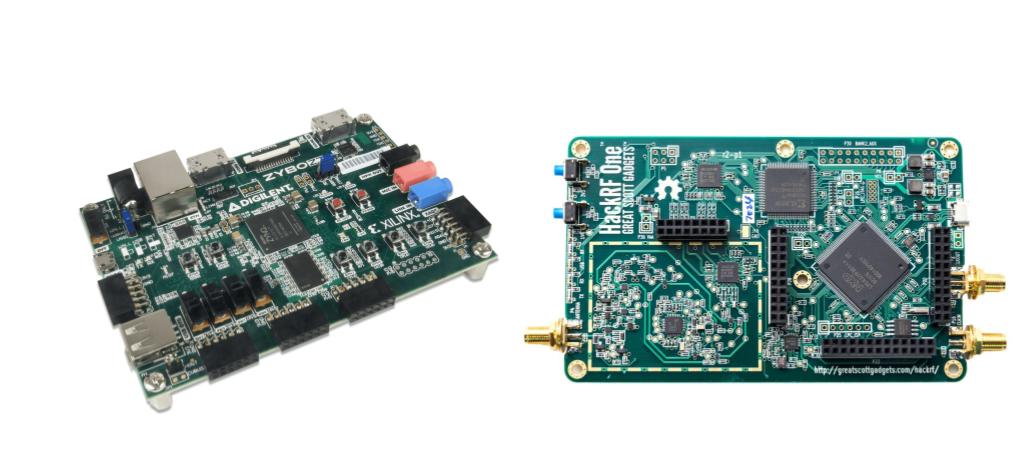
\includegraphics[width=3.5in]{images/zybohackrf.jpg} % adjust width as needed
  \caption{Zybo (Left), HackRF One (Right)}
  \label{fig:zybohackrf}
\end{figure}

The HackRF One is an open source SDR platform developed by Great Scott Gadgets. It is a half-duplex transceiver that operates from 1 MHz to 6 GHz, meaning it can both receive data and transmit
data in this band. The hardware is centered around an AD9361 RF transceiver chip that handles analog tasks, and an ARM Cortex-M4 microcontroller for digital tasks. It is powered and controlled
via USB, and can be interfaced with using the "libhackrf" API that is maintained by the developers. Using this API, the user can adjust parameters like center frequency, bandwidth, gain, etc.
The HackRF will operate at these user defined parameters, and provide baseband data of the signal serially over USB \cite{hackrf_docs,hackrf_repo}.

The ZYBO is a Zynq-based SoC development board designed by Digilent. The board is centered around a Xilinx Zynq-7000 series SoC, which features a dual-core ARM Cortex-A9 processor and programmable FPGA fabric. The Zybo also includes on-board peripherals like DDR memory, USB, HDMI, Ethernet, GPIO, etc. The programmable logic is programmed via Hardware Design Languages (HDL) in the Xilinx Vivado Suite, and the processing system is programmed in Embedded C using the Xilinx Vitis Suite. The two can communicate via an AXI interconnect, allowing for seamless integration of the processor and FPGA fabric \cite{digilent_zybo_manual}.

\subsection{System Overview}
\label{subsec:sysoverview}
\begin{figure}[htbp]
  \centering
  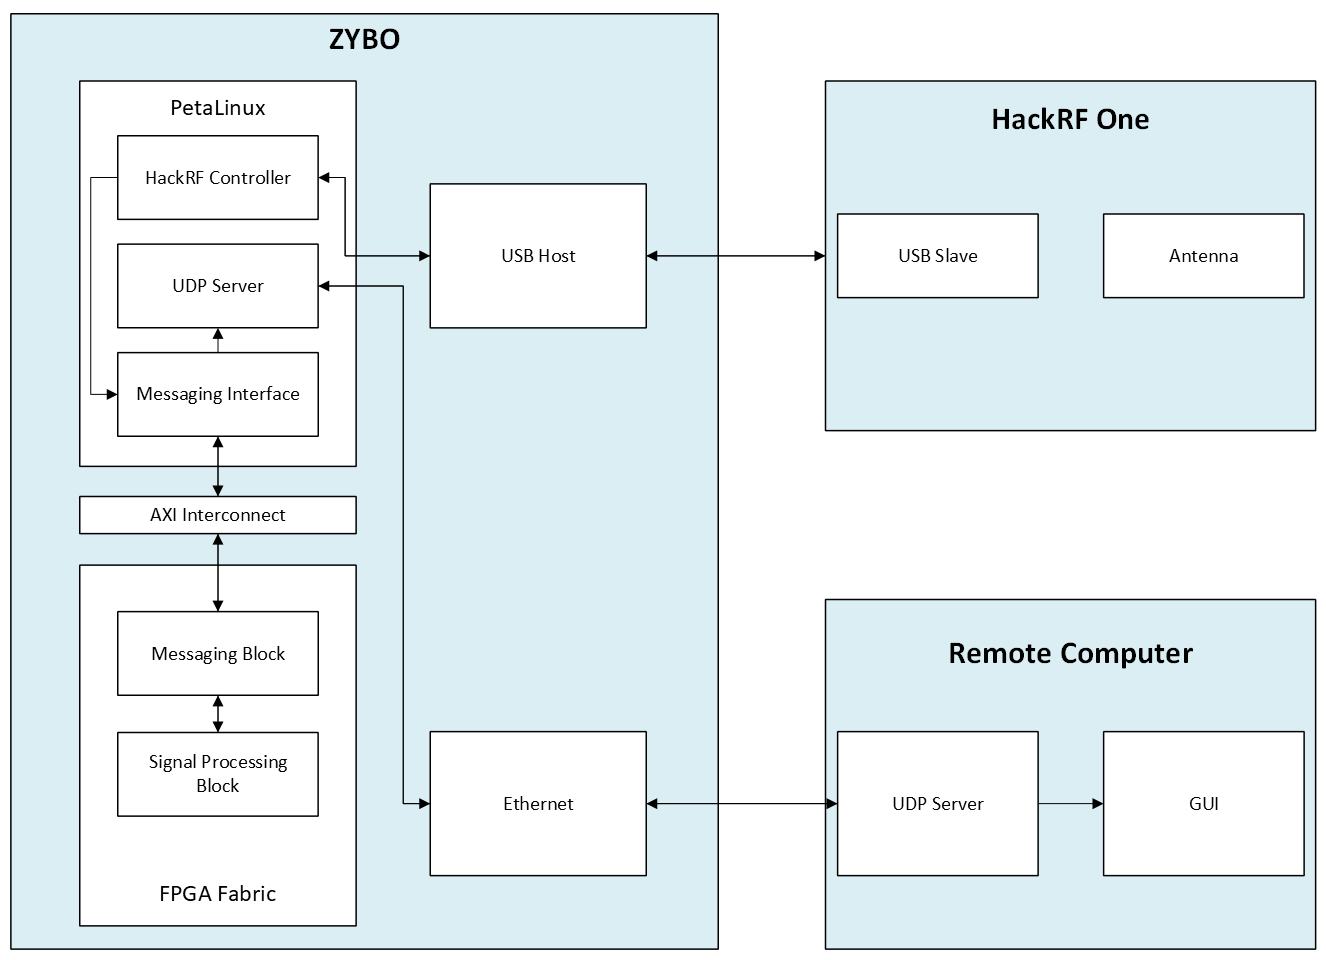
\includegraphics[width=3.5in]{images/systemdiagram.png} % adjust width as needed
  \caption{System Diagram of S(oC)DR}
  \label{fig:sysdiagram}
\end{figure}

To use the HackRF One and Zybo development boards to create a unified SoC and SDR development platform, a custom interface needs to be made for the Zybo that can control and communicate with the HackRF, use the data in the FPGA fabric for processing, and communicate this data to a computer for visualization and remote controlling. The implementation of this interface is laid out in Figure \ref{fig:sysdiagram}, which shows the blocks and connections necessary to fulfill these features. The Zybo features a USB On-The-Go (OTG) peripheral which can act as an embedded USB host that can both power and control the HackRF One. It also features an Ethernet port with a MAC controller which can be used as a method to send data over a network to a remote machine. Internally, an embedded Linux kernel can be ran on the Zybo's processor and dedicated DDR memory for abstracting the device drivers needed to operate these peripherals. It will also make developing custom software that can interface with these peripherals much easier than having to write bare metal software. The software that will reside in the Linux kernel will be a HackRF Controller, a UDP server, and a messaging interface. The HackRF controller will use the libhackrf API to establish a stream of data from the HackRF into the program, as well as allow for a simple way to control the HackRF's operating parameters. The data stream in the controller will be given to a messaging interface, which will be able to communicate with the FPGA fabric via an AXI interconnect that is baked into the SoC. The data received from the FPGA fabric after processing will then be sent to a UDP server, which will be able to interface with the Ethernet peripheral to send frames of signal data over the network to a client machine for further use. It can also accept data from a client that will be sent to the HackRF Controller to remotely control the HackRF. The FPGA fabric will have a similar messaging block for taking in and formatting data from the AXI interconnect. This messaging block will be packaged as an IP block with a generic and reusable interface so that users can design their own custom signal processing chains in HDL that can easily interface with the messaging block and abstract the complexities of communicating with the Linux kernel over AXI \cite{digilent_zybo_manual,hackrf_repo}. 

The deliverables for this project will be a Linux image that is pre-loaded with all the aforementioned software, as well as an editable Vivado project with the custom HDL that the user can edit to include their own signal processing chains. This will abstract all the complexities of having to interface between the Zybo and HackRF One development boards, and yield an extremely cost effective and powerful SoC and SDR development platform.

\subsection{Development Environment}
\begin{figure}[htbp]
  \centering
  \includegraphics[width=3.5in]{images/labsetup.jpg} % adjust width as needed
  \caption{Lab Setup}
  \label{fig:labsetup}
\end{figure}
The development environment consists of an Ubuntu 22.04 operating system, PetaLinux 2017.4 which uses the Yocto Project Version 2.2, and Vivado 2017.2. The actual hardware and lab setup is shown in Figure \ref{fig:labsetup}, with a Zybo connected to a HackRF One via USB and an Ethernet cable connecting it to a local router. The Zybo is powered with a dedicated power supply to provide enough amperage to power the HackRF One. Another USB cable is used between the Ubutnu machine and the Zybo to remote into the Zybo's embedded Linux shell. A wide-band dipole antenna is used with the HackRF One to capture data along its entire band.

\subsection{Linux Image}
\begin{figure}[htbp]
  \centering
  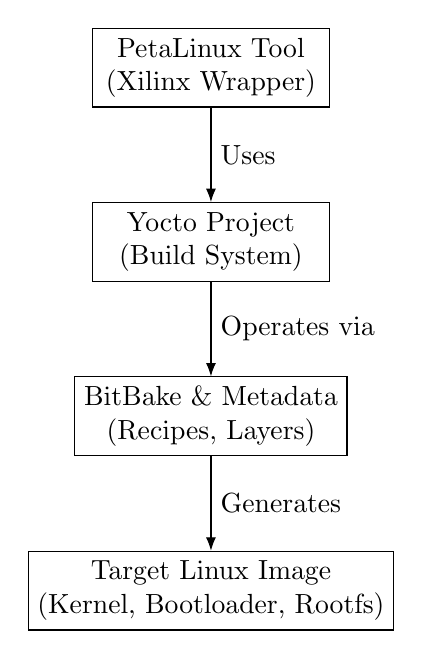
\begin{tikzpicture}[node distance=1.2cm, auto, >=Latex]
    % Nodes for PetaLinux wrapper diagram
    \node[draw, rectangle, align=center, minimum width=3cm, minimum height=1cm] (PL) {PetaLinux Tool\\ (Xilinx Wrapper)};
    \node[draw, rectangle, align=center, below=of PL, minimum width=3cm, minimum height=1cm] (YP) {Yocto Project\\ (Build System)};
    \node[draw, rectangle, align=center, below=of YP, minimum width=3cm, minimum height=1cm] (BB) {BitBake \& Metadata\\ (Recipes, Layers)};
    \node[draw, rectangle, align=center, below=of BB, minimum width=3cm, minimum height=1cm] (IMG) {Target Linux Image\\ (Kernel, Bootloader, Rootfs)};
    
    % Arrows for PetaLinux wrapper diagram
    \draw[->] (PL) -- node[right]{Uses} (YP);
    \draw[->] (YP) -- node[right]{Operates via} (BB);
    \draw[->] (BB) -- node[right]{Generates} (IMG);
\end{tikzpicture}
\caption{PetaLinux and Yocto}
\label{fig:petalinuxyocto}
\end{figure}

To deploy an embedded Linux kernel onto the Zybo, Xilinx has provided a toolkit called PetaLinux to help with the process for Xilinx specific targets, and its operation can be seen in Figure \ref{fig:petalinuxyocto}. Under the hood of PetaLinux is an open source build framework called Yocto, which uses other open source tools like BitBake, poky, and OpenEmbedded
to make it easy to build custom Linux images for a variety of targets. Yocto is a layered architecture, meaning users can define custom layers for each
library, piece of software, or device driver they want to add in the Linux image to allow for extremely granular control over the size and operation of the resulting Linux image. PetaLinux uses the Yocto project, and provides custom layers for Xilinx specific hardware like the Zynq-7000 series which is used in the Zybo. It also allows for a seamless integration between the Linux image and the FPGA fabric on Xilinx SoCs. After synthesizing a hardware platform for the FPGA fabric, an XSA file from the build artifacts can be used in PetaLinux to make sure the Linux image can interface with the hardware platform \cite{amd_petalinux_ug1144}.

\begin{figure}[htbp]
  \centering
  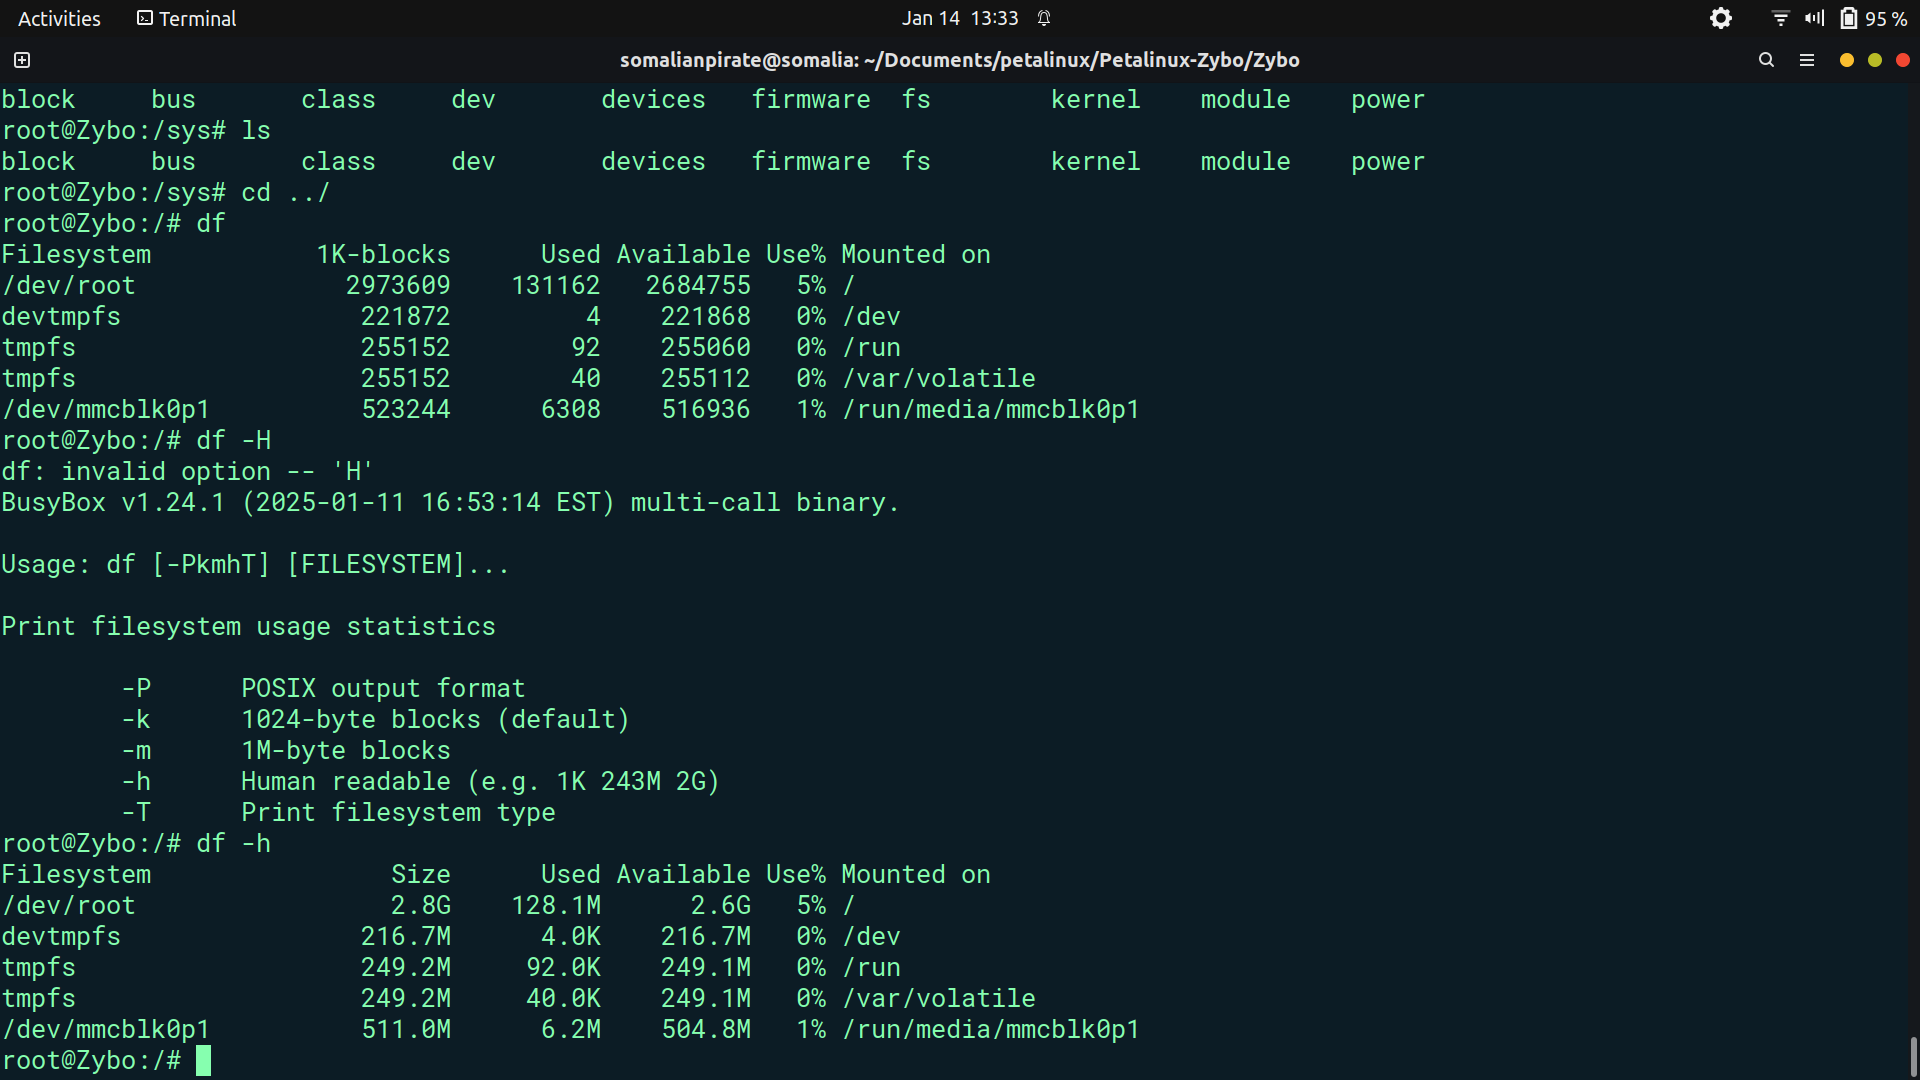
\includegraphics[width=3.5in]{images/linuxshell.png} % adjust width as needed
  \caption{Zybo Linux Shell}
  \label{fig:linuxshell}
\end{figure}

Digilent, the manufacturer of the Zybo, provides an example PetaLinux project and hardware platform that have pre-written device drivers and interfaces to use the board peripherals without any extra labor. Since this is open source, this is the starting point for this project in creating a Linux image and hardware platform that will include everything needed for an SoC and SDR platform. However, this example project was made in 2017, and has old dependencies and version conflicts that make it very hard to configure and build. After installing all the required dependencies, troubleshooting build errors, and making changes to Yocto layers, the example PetaLinux project was able to build and deploy onto the Zybo. In the final configuration of the PetaLinux project, an SD card is used to store the Linux kernel and the root filesystem to allow the DDR memory on the board to be completely dedicated to application memory. This will allow for a scalable size of storage space to store large chunks of signal data from the SDR, and as much memory as possible to run custom software. As can be seen in Figure \ref{fig:linuxshell}, remoting into the Zybo's Linux shell shows the proper configuration and build of an embedded Linux image targetted for the Zybo development board \cite{digilent_petalinux_zybo}.

\subsection{Meta-SDR and USB OTG Peripheral}
\begin{figure}[htbp]
  \centering
  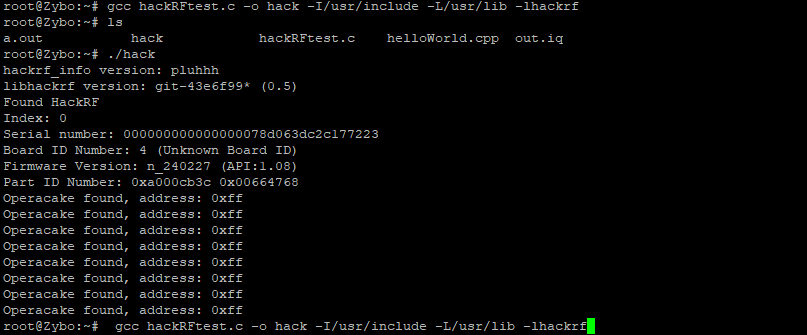
\includegraphics[width=3.5in]{images/meta_sdr.png} % adjust width as needed
  \caption{HackRF Info Tool from Meta-SDR}
  \label{fig:meta-sdr}
\end{figure}
Making custom software for an embedded ARM processor requires special compilation for the target, as most widely used compilers do not support embedded ARM architectures. Therefore, to use the HackRF libraries and other SDR tools this requires specific compilation of the libraries, and an inclusion of these compiled libraries into the root filesystem of the embedded linux environment. Thankfully, the OpenEmbedded community hosts open source Yocto layers that execute these steps for the developer in the Yocto build system. Meta-SDR is an OpenEmbedded layer which includes recipes, or scripts, for many popular SDR tools including the HackRF libraries. After tweaking the Meta-SDR layer to include a newer version of the HackRF library and modifying Yocto include files, the HackRF libraries and utilities were included into the root filesystem of the PetaLinux build \cite{meta_sdr_layer,amd_petalinux_ug1144}. To test their functionality, the source code for the "hackrf\_info" utility was copied into its own file on the embedded Linux target. The HackRF libraries in the root filesystem were linked during compilation, and the "hackrf\_info" utility compiled and ran successfully as can be seen in Figure \ref{fig:meta-sdr}. 

Since these HackRF utilities are now usable on the Zybo, this allowed for testing to be conducted on whether the HackRF can be powered and recognized from the USB OTG peripheral on the Zybo. USB On-The-GO (OTG) is a standard which allows embedded devices like smartphones or SoC development boards to act as USB hosts, essentially mimicing a standard desktop. The connection between the Zybo and HackRF using the USB OTG peripheral can be seen in Figure \ref{fig:labsetup}. A note in the peripheral's operation is that the HackRF requires up to 440 mA of current depending on its operation, meaning this peripheral must be able to supply this current at any given time. The Zybo reference manual states that the USB OTG peripheral can provide up to 500 mA of current through the peripheral only if the Zybo is powered from a wall supply. The implication of this is that the final system must utilize a bigger battery pack with an electrical outlet to enable this amount of current draw from the HackRF in a field environment. To test the data communication over this USB OTG peripheral, the "hack\_info" utility compiled and ran previously in Figure \ref{fig:meta-sdr} shows metadata being read from the HackRF such as serial number, firmware version, etc., showing a successful connection between the Linux kernel, the USB peripheral, and the HackRF \cite{digilent_zybo_manual,hackrf_docs}.

\subsection{Future Work}
Existing work created a working Linux environment with all the tools and libraries necessary for interfacing with the HackRF. Next, the software discussed in Section \ref{subsec:sysoverview} must be written and tested, including the HackRF Controller, UDP server, and Messaging Interface. As well this, an effort should be made to edit the Digilent Vivado project that is used in the current PetaLinux build to include a custom Messaging IP Block.

\nocite{*}
\bibliographystyle{ieeetr}  % Use IEEE format
\bibliography{refs}
\end{document}
